\documentclass[11pt,letterpaper]{article}
\usepackage[utf8]{inputenc}
\usepackage{amsmath,amssymb,fullpage,graphicx}
\usepackage{subfigure}
\let\hat\widehat
\let\tilde\widetilde

\begin{document}
\subsection*{Q3-a}
\noindent Posterior function on prior $Beta(1,1)$ can be written as
\begin{align*}
\pi(\theta | x) &\propto L(\theta | x)\pi(\theta)\\
&\propto \theta^{21} (1- \theta)^{68-21} \theta^{1 - 1} (1- \theta)^{1 - 1} \\
&\propto \theta^{22 - 1} (1 - \theta)^{48 - 1}
\end{align*}

\noindent The posterior follows $Beta(22, 48)$

\begin{verbatim}
theta <- seq(0, 1, 0.001)
post1 <- dbeta(theta, 469/18, 937/18)
post2 <- dbeta(theta, 22, 48)

plot(x=theta, y=post1, type='l', lwd=2, xlab='theta', ylab='posterior density', 
     main='Posterior Density with Different Priors')
lines(x=theta, y=post2, lty=3, lwd=2)
legend('topright', legend=c('Prior Beta(5.05, 5.05)', 'Prior Beta(1,1)'), 
       lty=c(1,3), lwd=3, cex=0.75)
\end{verbatim}

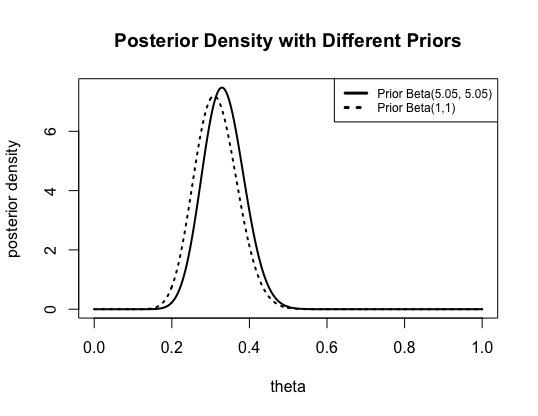
\includegraphics[width=150mm]{q3-a.png}

\noindent Two posterior distributions share identical general shape, since they are both Beta distributions. The variance of posterior with prior $Beta(1, 1)$ is slightly bigger and its median is smaller than the posterior with prior $Beta(5.05, 5.05)$.

\newpage
\subsection*{Q3-b}
\begin{verbatim}
upper <- qbeta(0.975, 22, 48)
lower <- qbeta(0.025, 22, 48)
> upper
[1] 0.4268747
> lower
[1] 0.2117479
\end{verbatim}

\noindent The $95 \%$ credible interval is [0.2117479, 0.4268747]. \\
\noindent Compare to the credible interval calculated in previous problem, this interval has lower values in both lower and upper bounds.


\end{document}